% =============================================================================
%  CAPA DO LIVRO (DESIGN EDITORIAL IMPACTANTE)
% =============================================================================
\begin{capa}
    \begin{tikzpicture}[remember picture, overlay]
        % Background
        \fill[gray!4] (current page.south west) rectangle (current page.north east);
        
        % Left decorative sidebars (asymmetrical aesthetic)
        \fill[blueaccent] (current page.north west) rectangle ($(current page.south west) + (2.2cm, 0)$);
        \fill[cyanaccent] ($(current page.north west) + (2.2cm, 0)$) rectangle ($(current page.south west) + (2.35cm, 0)$);
        
        % Top header block (Collection / Volume)
        \node[anchor=north west, text width=15cm, align=left] at ($(current page.north west) + (3.2cm, -2.5cm)$) {
            {\color{fgalt}\sffamily\fontsize{10}{12}\selectfont\bfseries\MakeUppercase{Coleção Tecnologia na Saúde}}\\[0.15cm]
            {\color{blueaccent}\sffamily\fontsize{11}{13}\selectfont\bfseries\MakeUppercase{Volume 2: Gêmeos Digitais Periodontais e o Framework SUS-Twin}}
        };
        
        % Main Title Block
        \node[anchor=north west, text width=15cm, align=left] at ($(current page.north west) + (3.2cm, -5.2cm)$) {
            {\color{fg}\sffamily\fontsize{34}{40}\selectfont\bfseries GÊMEOS DIGITAIS}\\[0.15cm]
            {\color{fg}\sffamily\fontsize{34}{40}\selectfont\bfseries PERIODONTAIS}\\[0.5cm]
            {\color{fgalt}\sffamily\fontsize{13}{16}\selectfont\bfseries O Framework SUS-Twin e a Simulação}\\[0.1cm]
            {\color{fgalt}\sffamily\fontsize{13}{16}\selectfont\bfseries Biomecânica Periodontal no SUS}
        };
        
        % Approach & Qualis A1 Badge
        \node[anchor=north west, text width=15cm, align=left] at ($(current page.north west) + (3.2cm, -10.5cm)$) {
            {\sffamily\fontsize{12}{15}\selectfont\bfseries\color{fg} Uma Abordagem Profunda e Tecnológica}\\[0.35cm]
            \tikz[baseline=(char.base)]\node[anchor=north west, draw=blueaccent, fill=blueaccent!8, text=blueaccent, thick, rounded corners=3pt, inner sep=5pt] (char) {\fontsize{9}{10}\selectfont\bfseries COMPILADO COM RIGOR CIENTÍFICO QUALIS A1};
        };
        
        % Blueprint engineering grid in the background of the image
        \draw[step=0.5cm, blueaccent!15, very thin] ($(current page.north west) + (7cm, -12cm)$) grid ($(current page.north west) + (17cm, -22cm)$);
        \draw[step=2.5cm, blueaccent!30, thin] ($(current page.north west) + (7cm, -12cm)$) grid ($(current page.north west) + (17cm, -22cm)$);
        
        % Scanner acquisition graphics
        \draw[blueaccent!25, thin] ($(current page.north west) + (12cm, -17cm)$) circle (2.0cm);
        \draw[blueaccent!20, dashed] ($(current page.north west) + (12cm, -17cm)$) circle (3.8cm);
        \draw[blueaccent!35, thin] ($(current page.north west) + (12.0cm, -17.0cm) - (4.5cm, 0)$) -- ($(current page.north west) + (12.0cm, -17.0cm) + (4.5cm, 0)$);
        \draw[blueaccent!35, thin] ($(current page.north west) + (12.0cm, -17.0cm) - (0, 4.5cm)$) -- ($(current page.north west) + (12.0cm, -17.0cm) + (0, 4.5cm)$);
        
        % Transparent holographic tooth image
        \node[anchor=center] at ($(current page.north west) + (12cm, -17cm)$) {
            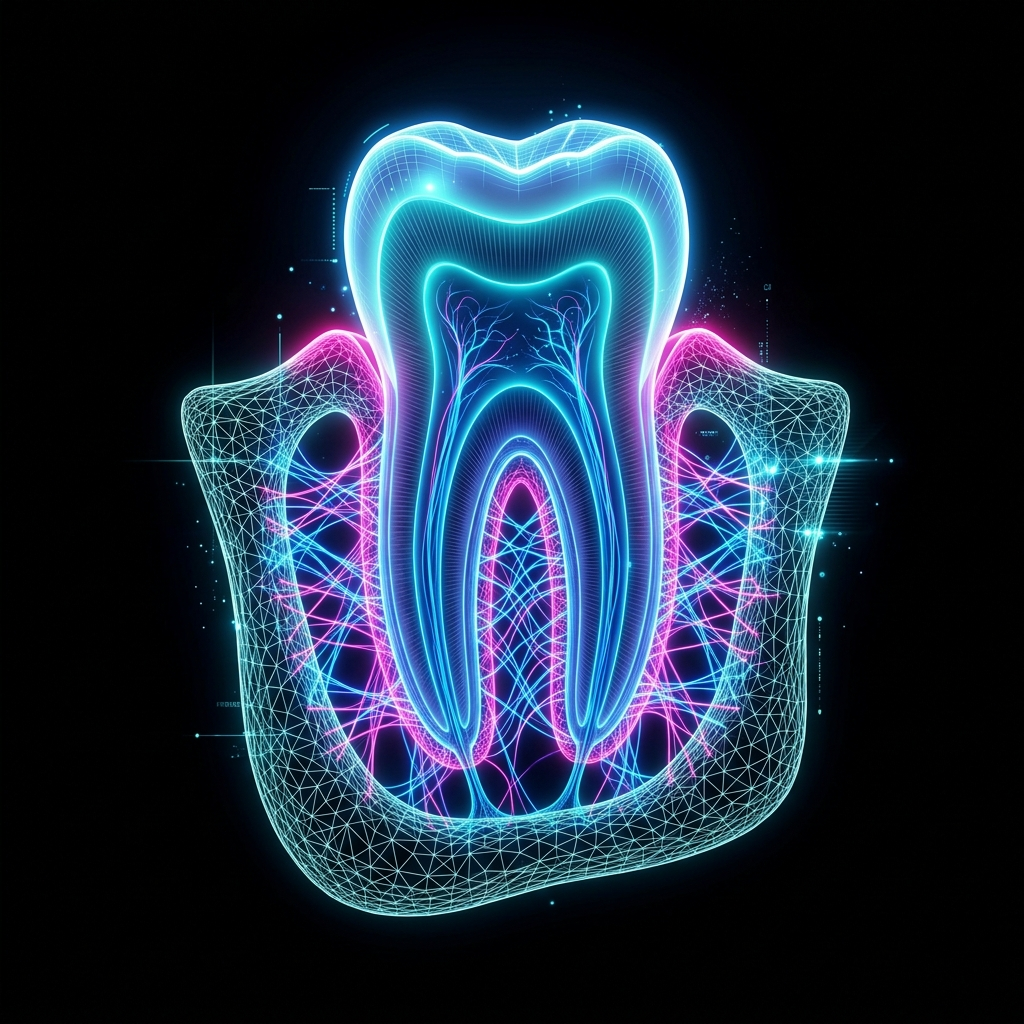
\includegraphics[width=8.5cm]{images/capa_logo_transparent.png}
        };
        
        % Author block
        \node[anchor=south west, text width=15cm, align=left] at ($(current page.south west) + (3.2cm, 3.8cm)$) {
            {\color{fg}\sffamily\fontsize{15}{18}\selectfont\bfseries Marcelo Claro Laranjeira}\\[0.15cm]
            {\color{fgalt}\sffamily\fontsize{9.5}{11}\selectfont\itshape Polímata e PhD --- Arquiteto-Chefe do OpenCode Ecosystem}
        };
        
        % Affiliation & Publisher block
        \node[anchor=south west, text width=15cm, align=left] at ($(current page.south west) + (3.2cm, 1.6cm)$) {
            {\color{fgalt}\sffamily\fontsize{8.5}{10}\selectfont\bfseries OpenCode Ecosystem Research Initiative}\\[0.05cm]
            {\color{fgalt}\sffamily\fontsize{8.5}{10}\selectfont Crateús, Ceará, Brasil ~|~ 2026}
        };
    \end{tikzpicture}
    \phantom{placeholder}
    \vfill
\end{capa}
